\begin{comment}
\section{Optimizations and enhancements}

 Task parallel programs that use mutual exclusion can have different computation graph structures based on the order in which the critical sections get executed. In this section, we discuss an algorithm to create all such computation graphs.
\end{comment}

\section{On-the-fly data race detection}
The data race detection technique presented in this work performs the analysis after the program has finished execution (post-mortem analysis). To improve the efficiency of analysis at run time, this paper presents a dynamic improvement for structured parallel programs. This technique is called on-the-fly data race detection.

The data race detection is run on a region as soon as \textbf{await} finishes execution on that region (i.e., \textsc{Await-done} fires). If no race is reported, all the nodes belonging to that region are merged into an equivalent master node that represents the region. The transformation preserves the partial order relative to other tasks. The variables accessed by the tasks in the region are added to the master node. 

\begin{figure}
  \begin{center}
    \begin{lstlisting}[mathescape=true]
  proc main(var n : int)
  	n := 1;
  	post $r_1 \leftarrow p_1~n~\varepsilon~\{r_1\}~\{r_1\}~\lambda v. n := n + v$;
	await $r_1$
 proc $p_1$(var n : int)
 	post $r_2 \leftarrow p_2~n~\varepsilon~\{r_1\}~\{r_1\}~\lambda v. n := n + v$;
  	post $r_2 \leftarrow p_3~n~\varepsilon~\{r_1\}~\{r_1\}~\lambda v. n := n + v$;  	  	
	await $r_2$
 proc $p_2$(var n : int)
	$\texttt{l}(r_2) := n$ 
 proc $p_3$(var n : int)
	$\texttt{l}(r_2) := n$
\end{lstlisting}
  \end{center}
    \vspace{-2em}
  \caption{Parallel program with nested regions.}
  \label{fig:nested-regions}
\end{figure}

\begin{figure}
  \centering
   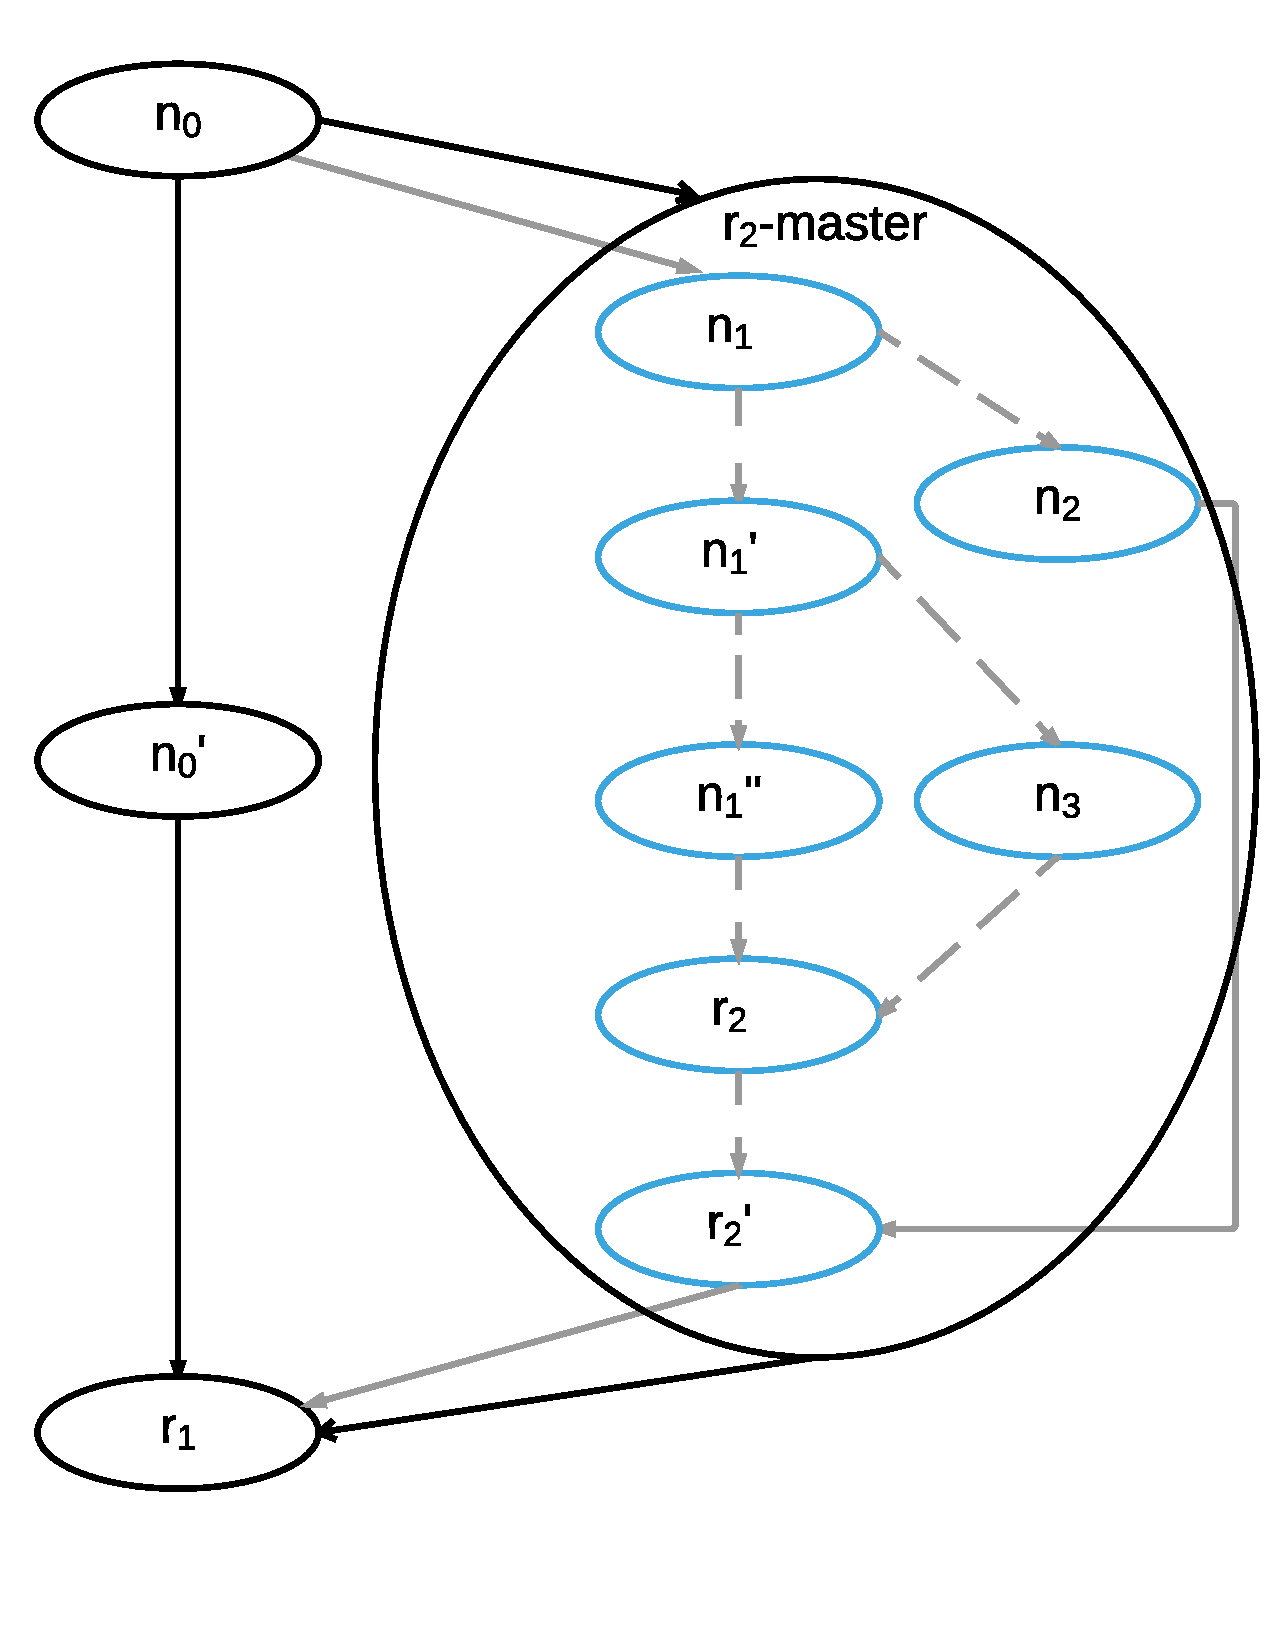
\includegraphics[width=0.35\textwidth]{../figs/Fig11.pdf}
   \vspace{-1em}
  \caption{Computation graph of example in \figref{fig:nested-regions}.}
        \vspace{-1em}
   \label{fig:cg-nested-regions}
\end{figure}

\figref{fig:nested-regions} shows an example of a parallel program with nested regions. As soon as the \textbf{await} on region $r_2$ finishes execution, on-the-fly analysis is run on this region to check for data races in the nodes belonging to this region. If a race is not reported, a master node is added to the graph that represents region $r_2$ and the program is executed further. The computation graph for this example is shown in \figref{fig:cg-nested-regions}. The nodes highlighted in blue with dashed lines denote the sub-graph that is replaced by a master node if the region is data race free.

\section{Mutual Exclusion}

\begin{figure*}
  \begin{center}
    \mprset{flushleft}
    \begin{mathpar}
     \and
      \inferrule[Isolated]
                {
				  \mathrm{canIsolate(C)} = \mathit{true} \\
                  n^\prime = \mathrm{fresh}() \\
                  N = N \cup \{n^\prime\} \\
                  E = E \cup \{\tuple{n, n^\prime},  \tuple{\mathit{last},n^\prime}\}\\
                }
{C[\tuple{\ell^\prime,S[\textbf{isolated}~s],\vec{r_\delta}^\prime,\vec{r_\omega}^\prime,d^\prime, n, 0}, m] \rightarrow
                  C[\tuple{\ell^\prime,
				   S[s; \textbf{isolated-end}],\vec{r_\delta}^\prime,\vec{r_\omega}^\prime,d^\prime, n^\prime, 1}, m]
                }
\and
      \inferrule[Isolated-Nested]
                {\mathit{iso} > 0 \\
                  \mathit{iso}^\prime = \mathit{iso} + 1
                }
{C[\tuple{\ell^\prime,S[\textbf{isolated}~s],\vec{r_\delta}^\prime,\vec{r_\omega}^\prime,d^\prime, n, \mathit{iso}}, m] \rightarrow
                  C[\tuple{\ell^\prime,
				   S[s; \textbf{isolated-end}],\vec{r_\delta}^\prime,\vec{r_\omega}^\prime,d^\prime, n, \mathit{iso}^\prime}, m]
}
\and
      \inferrule[Isolated-End-Nested]
                {\mathit{iso} > 1 \\
                  \mathit{iso}^\prime = \mathit{iso} - 1
                }
{C[\tuple{\ell^\prime,S[\textbf{isolated-end}],\vec{r_\delta}^\prime,\vec{r_\omega}^\prime,d^\prime, n, \mathit{iso}}, m] \rightarrow
                  C[\tuple{\ell^\prime,
				   S[\textbf{skip}],\vec{r_\delta}^\prime,\vec{r_\omega}^\prime,d^\prime, n, \mathit{iso}^\prime}, m]
                }
\and
      \inferrule[Isolated-End]
                {
                  n^\prime = \mathrm{fresh()}\\
                  \mathit{last} = n \\
                  N = N \cup \{n^\prime\} \\
                  E = E \cup \{\tuple{n, n^\prime}\}
                }
{C[\tuple{\ell^\prime,S[\textbf{isolated-end}],\vec{r_\delta}^\prime,\vec{r_\omega}^\prime,d^\prime, n, 1}, m] \rightarrow
                  C[\tuple{\ell^\prime,
				   S[\textbf{skip}],\vec{r_\delta}^\prime,\vec{r_\omega}^\prime,d^\prime, n^\prime,0}, m]
                }

\end{mathpar}
  \end{center}
  \caption{The transition rules for isolated statements.}
  \label{fig:isol-semantics}
\end{figure*}

Programs that use mutual exclusion to protect accesses to shared variables can have different computation graphs based on access order. All of these computation graphs have to be enumerated and analyzed for conflicting accesses outside of mutual exclusion.

The task parallel language is extended to model mutual exclusion with a new statement: $\textbf{isolated}~s$.
The statement performs $s$ in mutual exclusion of any other isolated statements. The semantics with how the computation graph is impacted is in \figref{fig:isol-semantics}. The isolation is accomplished by creating a new global variable \textit{last} to track the last node in the computation graph belonging to an isolated statement, by adding to the task context a counter initialized to zero to count the number of nested isolated contexts, and with a new keyword for the rewrite rules: \textbf{isolated-end}. 

Let $\mathrm{canIsolate}(C)$ be a function over configurations to Boolean that returns true for a configuration tree if all the task counters are 0; otherwise it returns false. If no other isolated statements are running, then the \textsc{Isolated} rule increments the task counter to indicate isolation and inserts after the isolated statement $\mathit{s}$ the new \textbf{isolated-end} keyword. The computation graph gets a new node to track accesses in the isolated statement with an appropriate edge from the previous node. A sequencing edge from $\mathit{last}$ is also added so the previous isolated statement happens before this new isolated statement. As a note, $\mathit{last}$ is initialized to an empty node when execution starts. The \textsc{Isolated-Nested} rule simply increments the counter if the task is already in isolation.

The \textsc{Isolated-End-Nested} rule processes the new \textbf{isolated-end} keyword and decrements the counter. When the counter reaches the outer-most isolated context, the \textsc{Isolated-End} rule creates a new node in the computation graph to denote the end of isolation, and it updates $\mathit{last}$ to properly sequence any future isolation. As a note, the on-the-fly data race detection is modified to not reduce sub-graphs with isolation.

\begin{algorithm}
\caption{Scheduling algorithm for Isolated blocks} \label{algo:isolated}
\begin{algorithmic}[1]
  \Function{schedule}{$t$, $\mathtt{Regs}$, $\mathtt{Tasks}$}
  \State \texttt{loop}:\ ($\mathtt{Regs}$, $\mathtt{Tasks}$) $:=$ \texttt{run}($t$, $\mathtt{Regs}$, $\mathtt{Tasks}$)\label{loc:run}
  \State $s :=$ \texttt{status}($t$)
  \State $R :=$ \texttt{runnable}($\mathtt{Tasks}$)
  \If{ $s =$ ISOLATED}\label{loc:entry:isolated}
  \ForAll{$t_i \in R$}\label{loc:prsched}
  \State \texttt{schedule}($t_i$, $\mathtt{Regs}$, $\mathtt{Tasks}$)
  \EndFor
  \Else
  \State $t_i$ := \texttt{random}($R$)\label{loc:rand}
  \State \texttt{schedule}($t_i$, $\mathtt{Regs}$, $\mathtt{Tasks}$)
  \EndIf
  \EndFunction
\end{algorithmic}
\end{algorithm}

Algorithm \ref{algo:isolated} presents a scheduling algorithm to enumerate all computation graphs resulting from isolation \cite{mercer2015model}. The algorithm considers a simplified state of the program with $\mathtt{Regs}$ being the set of region variables that are shared among the tasks, $\mathtt{Tasks}$ being the set of tasks, $t$ being a task, and $R$ being the set of runnable tasks. The algorithm also implements sequential semantics where only one task runs at a time and that task runs until it waits, completes, or isolates at which time a scheduling choice is made. Sequential semantics are viable  by \lemmaref{lem:drf} and \corref{cor:drf} that establish independence in the computation graph and execution schedule in the absence of data races. 

Line 2 updates the region variables and pool of tasks by running task $t$ until it exits, waits, or reaches an \textbf{isolated}-construct. The function \texttt{status} on Line 3 returns the status of the task $t$. On Line 4, the function \texttt{runnable} is used to obtain a list of all the tasks that can be run from the pool of all tasks. If the status of the currently running task $t$ becomes ISOLATED (i.e., the task encounters an \textbf{isolated} construct), the task is preempted and all the tasks that are runnable, including the task that is trying to isolate, are scheduled by the runtime. When the task completes, a new task is randomly selected from the set of runnable tasks.

\begin{figure}
  \begin{center}
    \begin{lstlisting}[mathescape=true]
  proc main(var n : int)
  	n := 1;
  	post $r_1 \leftarrow p_1~n~\varepsilon~\{r_1\}~\{r_1\}~\lambda v. n := n + v$;
  	post $r_1 \leftarrow p_2~n~\varepsilon~\{r_1\}~\{r_1\}~\lambda v. n := n + v$;
  	await $r_1$
 proc $p_1$(var n : int)
 	isolated $\texttt{l}(r_1) := n + 1$
 proc $p_2$(var n : int)
	isolated if $(\texttt{l}(r_1) = n)$ then
	  	post $r_1 \leftarrow p_3~n~\varepsilon~\{r_1\}~\{r_1\}~\lambda v. n := n + v$;
	else
		$\texttt{l}(r_1) := n - 1$
 proc $p_3$(var n : int)
	$\texttt{l}(r_1) := n+2$
\end{lstlisting}
  \end{center}
  \vspace{-1em}
  \caption{Parallel Program with Mutual exclusion.}
  \vspace{-1em}
  \label{fig:hj-isolated}
\end{figure}

\begin{figure}
  \centering
  \subfigure[p2 runs before p1.]{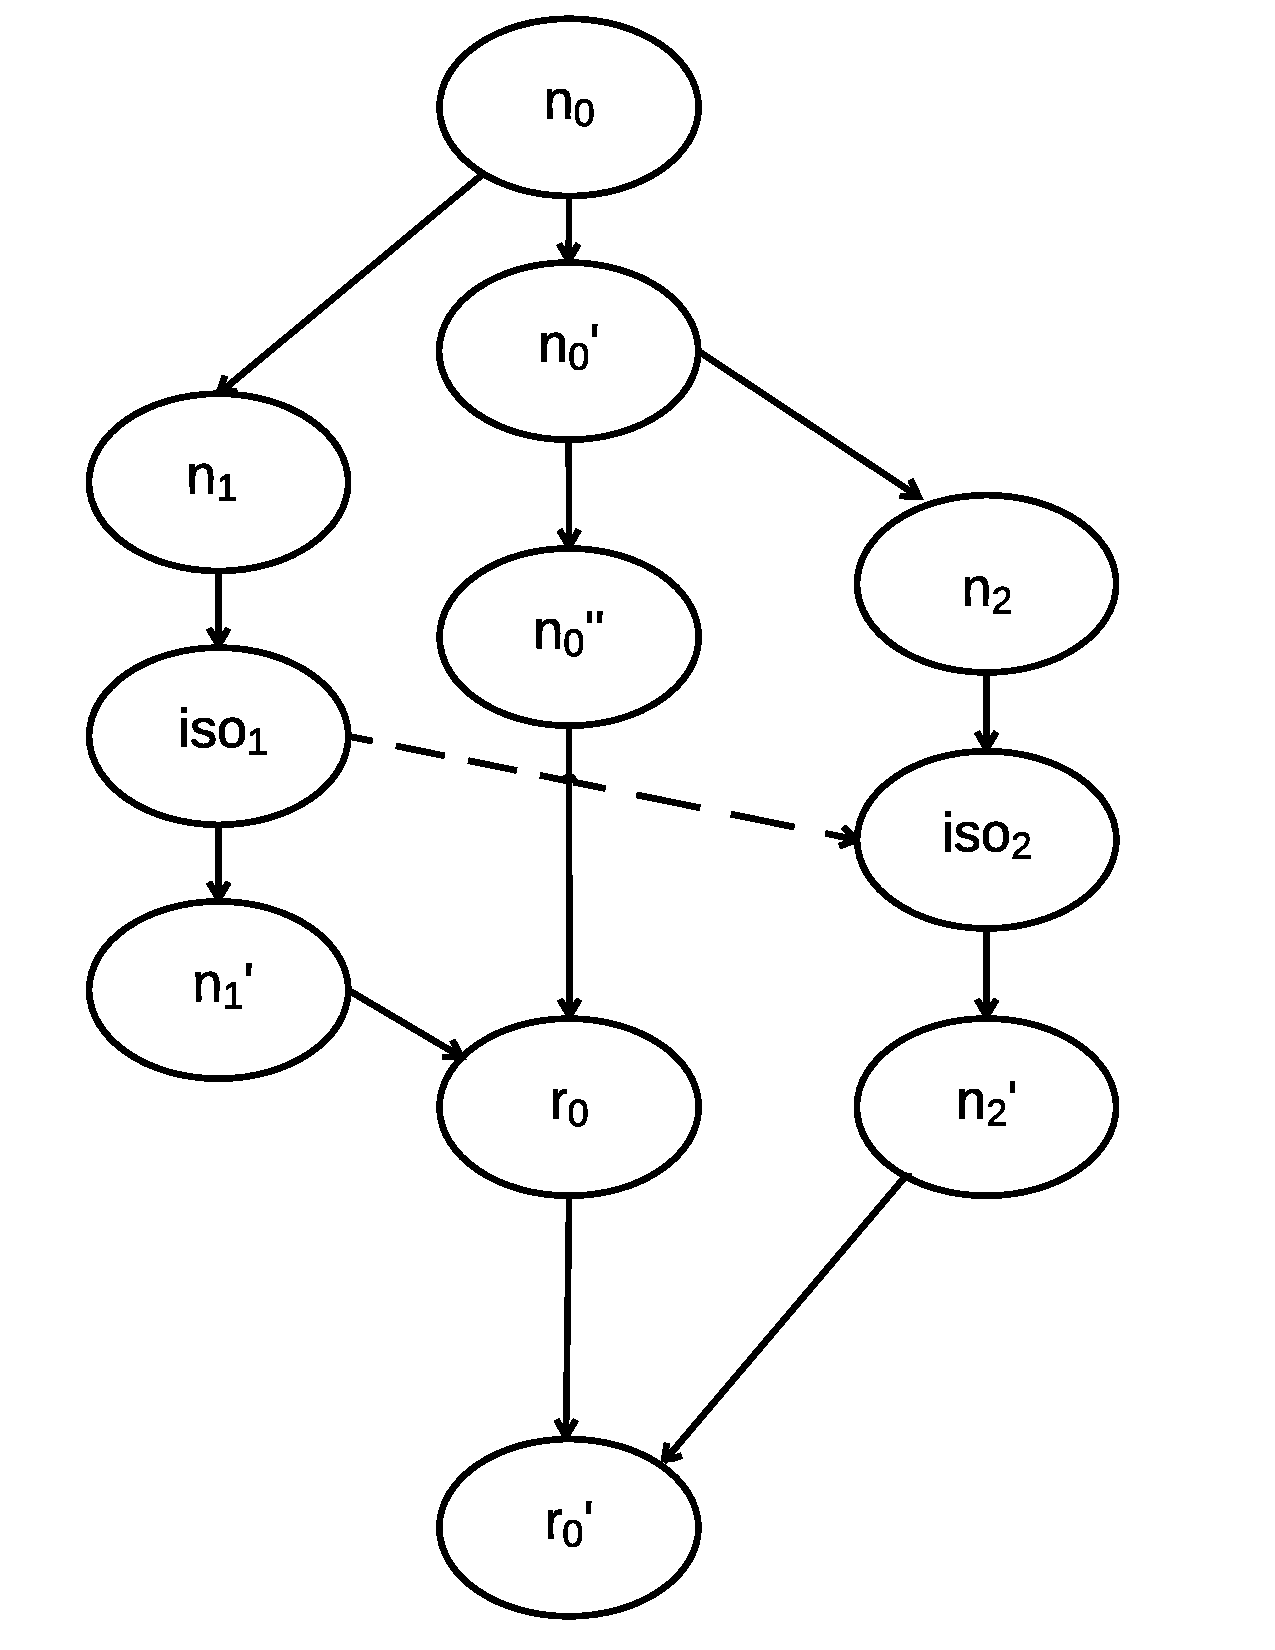
\includegraphics[scale=0.2]{../figs/Fig5-a.pdf}}
  \subfigure[p1 runs before p2.]{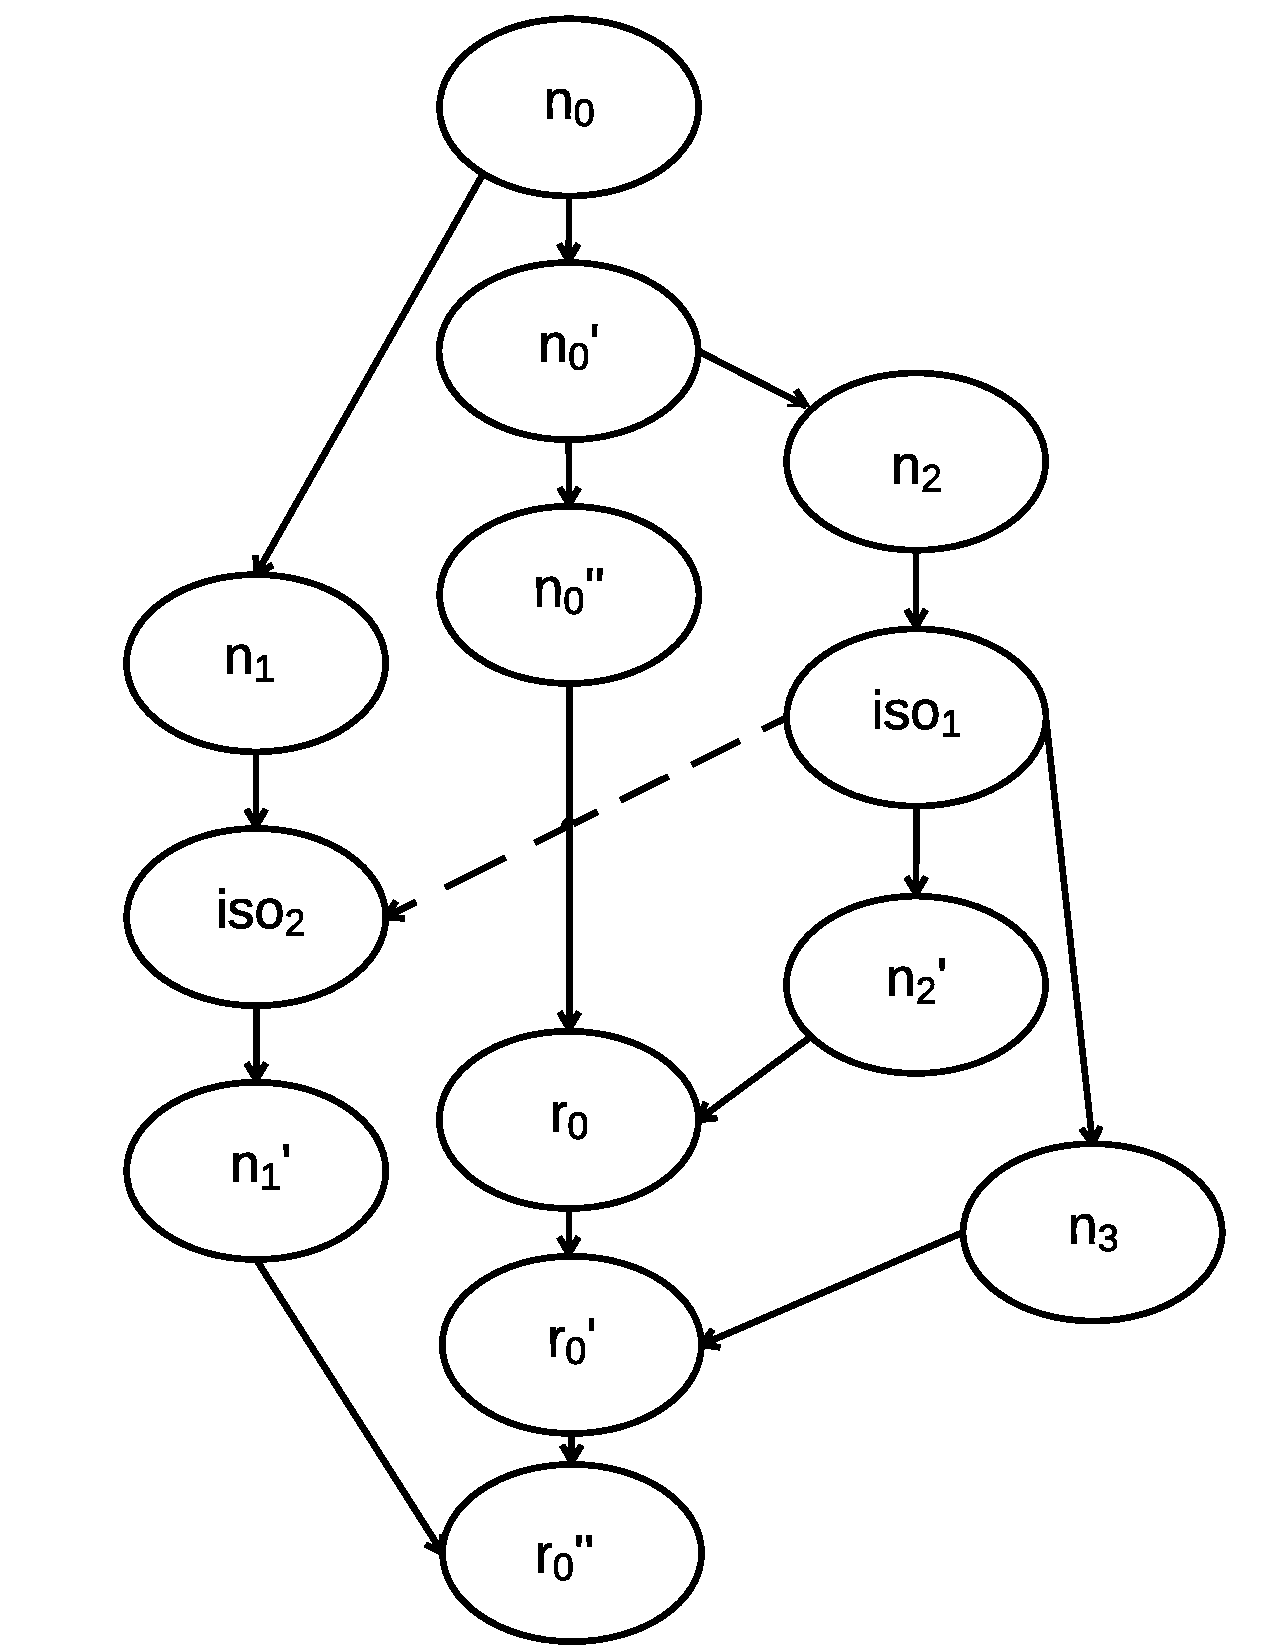
\includegraphics[scale=0.2]{../figs/Fig5-b.pdf}}
  \caption{Computation graphs of example in \figref{fig:hj-isolated}}
  \vspace{-1em}
   \label{fig:cg-isolated}
\end{figure}

For the example in \figref{fig:hj-isolated}, two different computation graph structures can be formed based on the order of execution of isolated blocks. The computation graphs are shown in \figref{fig:cg-isolated}. If the scheduler runs the isolated section of task $t_1$ first, the computation graph in \figref{fig:cg-isolated}(a) is formed. Task $t_1$ changes the values of shared variable $r_1$ to 2. Hence, when task $t_2$ executes its isolated section, the if-condition fails and an additional task is not spawned by $t_2$. If the scheduler runs task $t_2$ first, the computation graph of \figref{fig:cg-isolated}(b) is formed. In this schedule, task $t_2$ executes its isolated section first. Since the value of variable $r_1$ is 1, the if-condition is met and a new task is created by $t_2$.

\begin{theorem}
\algoref{algo:isolated} finds all unique computation graphs for structured parallel programs with isolated sections making it sound and complete with \algoref{algo:drd}.
%\algoref{algo:drd} is sound and complete for structured parallel programs with mutual exclusion.
\end{theorem}

\begin{proof}
%Theorem \ref{thm:strcutured-par-progs} states that Algorithm \ref{algo:drd} is sound and complete for structured parallel programs that do not contain isolated sections. If mutual exclusion is present, Algorithm \ref{algo:drd} does not remain sound since different computation graph structures can be formed for such programs. Algorithm \ref{algo:isolated} helps to enumerate all such computation graph structures. Therefore, the data race detection using Algorithm \ref{algo:drd} becomes sound and complete when it is used along with Algorithm \ref{algo:isolated} for structured parallel programs that have mutual exclusion.
From \thmref{thm:strcutured-par-progs} and \algoref{algo:isolated}, \algoref{algo:drd} is sound and complete for structured parallel programs with mutual exclusion.
\end{proof}
